% 附录 AB：空间与天体等离子体——从太阳风到磁层与重联（v1.26.6 新增）
% 数值唯一来源：tools/calc/appAB_calc.py -> tools/calc/appAB_calc.txt（正文数字的唯一来源；检查项 P34）
% 单位写法：km/s / nT / Pa / W / s / R_E，全部走 \mathrm{}，不放中文字符进数学字体。
% 版权口径：只借鉴经典教材与文献的物理结论、公式形式与题型；文字、数值与表格自拟并独立复算。
% 本书不列 DOI，只给书名、作者、年份、卷期页。
% 分工：M--AA 讲的是托卡马克主线（加热、边界、约束、增益、破裂、快粒子、辐射、强场、堆工程、替代位形）；
%       本附录跳出实验室，讲太阳风—磁层—重联这条天体链，重点是「同一套方程，两套尺度」。
% 引用的全部数字由 tools/calc/appAB_calc.py 现算；脚本内声明的输入见 AB.2 开头的表。

\section{四个尺度：从太阳风到磁尾}
\label{sec:app-ab-scales}
\setlength{\emergencystretch}{3em}

前面二十几个附录讲的全是\textbf{实验室里的等离子体}：装置在几米到几十米，时间在毫秒到秒。
本附录换一套尺度：太阳风的尺度是 $10^{11}\ \mathrm{m}$，磁层的尺度是 $10^{7}\ \mathrm{m}$，
而决定它们行为的仍然是同一套方程——磁流体力学加动理学修正。
唯一真正变化的是\textbf{碰撞}：在实验室里粒子碰得足够多，在天体里粒子几乎不碰。

把这条链摆在四个数上：

\begin{equation}
\frac{\text{太阳风}}{\text{磁层}}=\frac{10^{11}\ \mathrm{m}}{10^{7}\ \mathrm{m}}
=10^{4},\qquad
\frac{\text{离子回旋半径}}{\text{装置尺度}}\ll 1 .
\label{eq:app-ab-scales}
\end{equation}

第一个数是空间尺度之比：太阳风把整个磁层当成一个「小障碍物」绕过去。
第二个数才是关键：只要离子回旋半径远小于边界尺度，\textbf{单流体描述就成立}，
磁层顶才能被当成一张「面」来处理；一旦这个比不再小，就要退回动理学。

\begin{table}[htbp]
\centering
\small
\begin{tabular}{p{2.4cm}p{3.4cm}p{3.4cm}p{4.2cm}}
\toprule
区域 & 特征尺度 & 特征时间 & 主导物理 \\
\midrule
太阳风 & $1\ \mathrm{AU}=1.496\times10^{11}\ \mathrm{m}$ & 输运 $4$ 天量级 & 无碰撞、超声速、冻结 \\
磁层 & $10\ R_E\approx6.4\times10^{7}\ \mathrm{m}$ & 对流 $10\ \mathrm{min}$ 量级 & 磁压主导、$\beta<1$ \\
电离层 & $100\ \mathrm{km}$ 厚 & 电导响应 $1\ \mathrm{s}$ 量级 & 有碰撞、佩德森电导 \\
磁尾 & $100\ R_E$ 长 & 亚暴 $1\ \mathrm{h}$ 量级 & 重联驱动、储能释放 \\
\bottomrule
\end{tabular}
\caption{空间等离子体的四个尺度。本附录只算前两行与最后一行，电离层只作为边界条件出现。}
\label{tab:app-ab-scales}
\end{table}

\begin{tip}{四个尺度不是四个数量级，是四种物理}{tip-app-ab-scales}
尺度差四个数量级只是表象。真正把人逼回动理学的是\textbf{碰撞平均自由程}：
太阳风在 $1\ \mathrm{AU}$ 里的平均自由程比 $1\ \mathrm{AU}$ 还长，
所以「温度」这种靠碰撞定义的概念在那里要打折扣——同一句话在实验室里是定义，在那里是假设。
\end{tip}

{\footnotesize
\textbf{出处：}本节的分区口径与尺度取值参照 Kivelson \& Russell \emph{Introduction to Space Physics}
（1995，第 1--3 章）与 Baumjohann \& Treumann \emph{Basic Space Plasma Physics}（1996，第 1 章）。
表 \ref{tab:app-ab-scales} 的四行内容由本文自拟，其中的量级关系都能用
所有文字、数值与表格均不复制原书，
只借鉴结论与讲解顺序。
}

\section{太阳风：为什么它是超声速的}
\label{sec:app-ab-solarwind}

给定一个工作点：密度 $n=5\ \mathrm{cm^{-3}}$、温度 $T=10\ \mathrm{eV}$、磁场 $B=5\ \mathrm{nT}$、
速度 $v=400\ \mathrm{km\,s^{-1}}$。这四个数就是本附录的全部输入。

先算两个频率。电子等离子体频率

\begin{equation}
\omega_{pe}=\sqrt{\frac{n e^2}{\varepsilon_0 m_e}}
=1.26147\times10^{5}\ \mathrm{rad\,s^{-1}}\;(20.08\ \mathrm{kHz}),
\label{eq:app-ab-omegape}
\end{equation}

离子的是 $\omega_{pi}=2943.89\ \mathrm{rad\,s^{-1}}\;(468.5\ \mathrm{Hz})$，比电子低 $42.9$ 倍——
这个比值只由质量比决定，和天体、实验室无关。

再算两个速度。声速

\begin{equation}
c_s=\sqrt{\frac{\gamma k_BT}{m_i}}
=43.769\ \mathrm{km\,s^{-1}},
\label{eq:app-ab-cs}
\end{equation}

阿尔芬速

\begin{equation}
v_A=\frac{B}{\sqrt{\mu_0\rho}}
=48.773\ \mathrm{km\,s^{-1}},
\label{eq:app-ab-va}
\end{equation}

其中质量密度 $\rho=8.36311\times10^{-21}\ \mathrm{kg\,m^{-3}}$ 由 $n$ 与质子质量算出。
两个速度只差一成（$c_s/v_A=0.89741$，即 $c_s$ 比 $v_A$ 低 $10.3\%$）——这是太阳风的\textbf{巧合}，
却正好让两个马赫数都不小：

\begin{equation}
M_s=\frac{v}{c_s}=9.1388,\qquad M_A=\frac{v}{v_A}=8.2012 .
\label{eq:app-ab-ms}
\end{equation}

\begin{equation}
\beta=\frac{2\mu_0 n k_BT}{B^2}=0.80534 .
\label{eq:app-ab-beta}
\end{equation}

\begin{table}[htbp]
\centering
\small
\begin{tabular}{p{3.4cm}p{3.0cm}p{3.0cm}p{4.0cm}}
\toprule
量 & 数值 & 单位 & 说明 \\
\midrule
电子等离子体频率 & $1.26147\times10^{5}$ & $\mathrm{rad\,s^{-1}}$ & $20.08\ \mathrm{kHz}$ \\
离子等离子体频率 & $2943.89$ & $\mathrm{rad\,s^{-1}}$ & $468.5\ \mathrm{Hz}$ \\
声速 & $43.769$ & $\mathrm{km\,s^{-1}}$ & $\gamma=1$，质子质量 \\
阿尔芬速 & $48.773$ & $\mathrm{km\,s^{-1}}$ & 用 $n$ 算出的质量密度 \\
声速马赫数 & $9.1388$ & --- & 超声速 \\
阿尔芬马赫数 & $8.2012$ & --- & 超阿尔芬速 \\
等离子体 $\beta$ & $0.80534$ & --- & 磁压与热压同量级 \\
\bottomrule
\end{tabular}
\caption{太阳风工作点的七个导出量。所有数由 \texttt{tools/\allowbreak{}calc/\allowbreak{}appAB\_calc.py} 现算。}
\label{tab:app-ab-solarwind}
\end{table}

\begin{tip}{太阳风超声速，靠的不是加热，是边界条件}{tip-app-ab-sonic}
$M_s=9.1388$ 不能理解成「太阳风被加热到了 9 倍声速」。
日冕的声速只有 $43.769\ \mathrm{km\,s^{-1}}$，而太阳风以 $400\ \mathrm{km\,s^{-1}}$ 流出去——
\textbf{超声速是解的性质}：日冕底部压力高、外部压力低，
流体解必须穿过声速点才能把压力放掉，于是太阳风在 $10\ R_\odot$ 附近自然加速到超声速。
这就是为什么地球附近永远量到 $M_s\approx9$，而不是「有时超声速、有时亚声速」。
\end{tip}

{\footnotesize
\textbf{出处：}本节公式与讲解顺序参照 Baumjohann \& Treumann \emph{Basic Space Plasma Physics}
（1996，第 1、8 章）与 Parks \emph{Physics of Space Plasmas}（2004，第 1--3 章）。
「声速点」的定性图像参照 Parker 的太阳风解（文献综述见 Kivelson \& Russell 1995，第 4 章）。
本节只借鉴结论与推导形式，公式里的四个输入取本附录的工作点，全部数值由
\texttt{tools/\allowbreak{}calc/\allowbreak{}appAB\_calc.py} 复算，不复制原书表格与文字。本附录\textbf{不复制}任何教材的数值表格。
}

\begin{figure}[htbp]
\centering
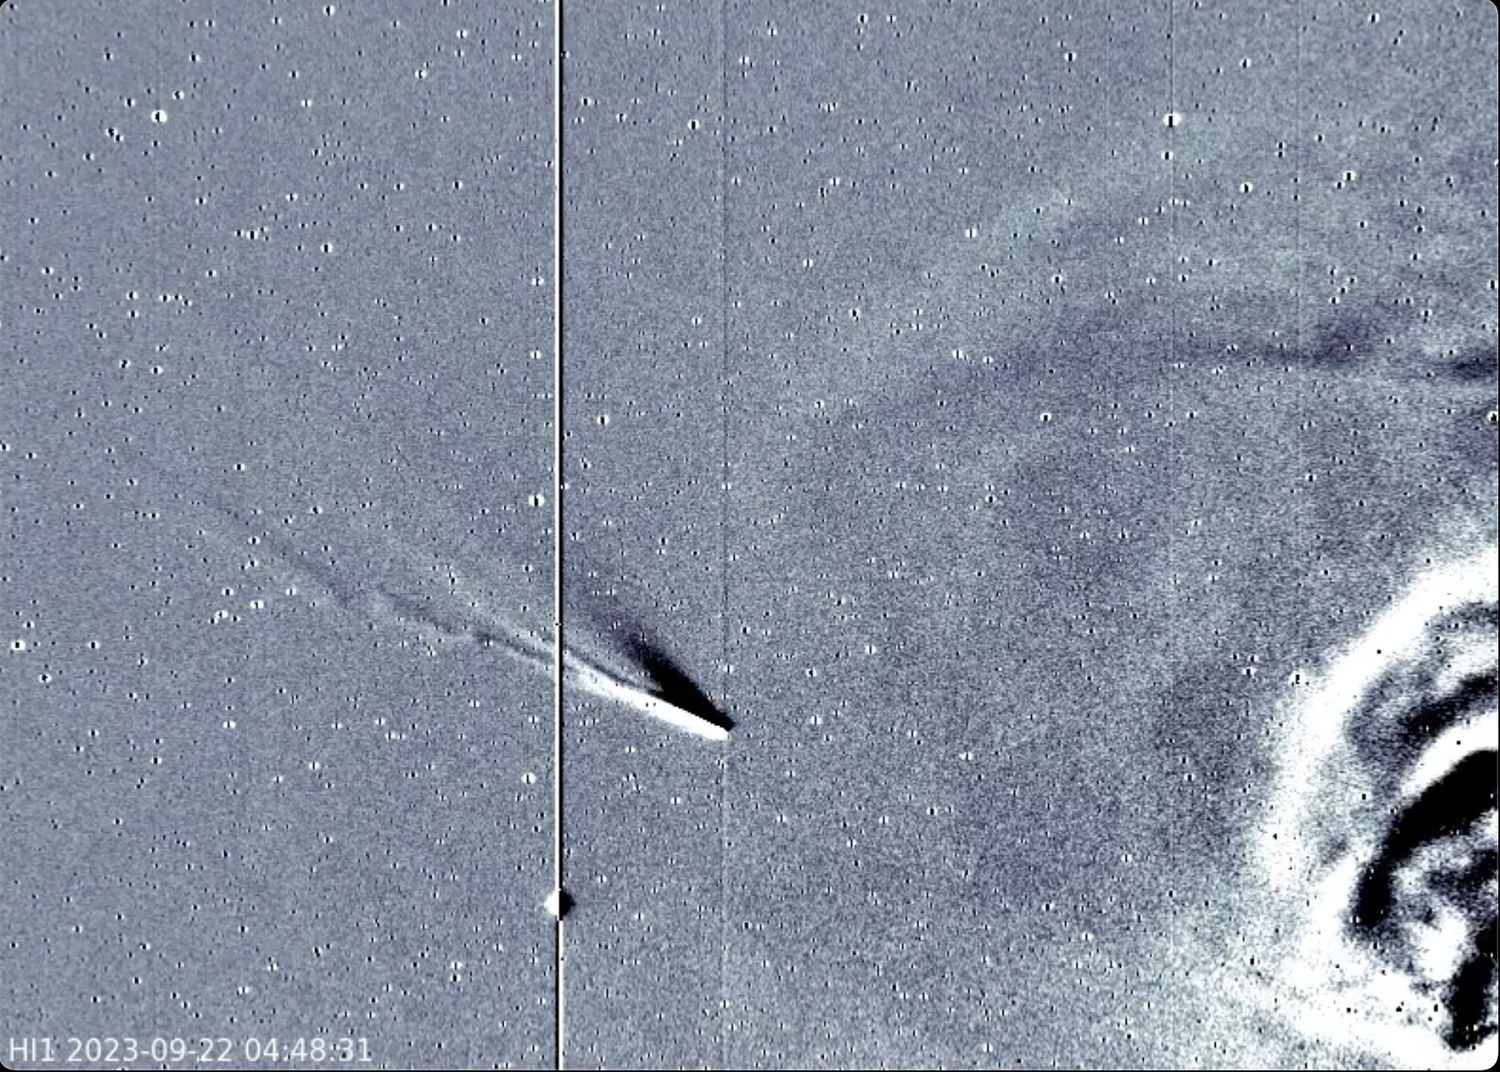
\includegraphics[width=0.72\textwidth]{../figures/ab_comet_ion_tail.jpg}
\caption{西村彗星的离子尾：太阳风吹过彗发，把离子拉成一条笔直的尾巴；尾巴一旦被太阳风里的扰动扫过，就会整条弯折。彗星因此是一支免费的“太阳风探针”——看不见的太阳风，在彗尾的形状上现了形。}
\label{fig:photo-appab2}
\figsource{STEREO / NASA（内日球成像仪 HI-1），Public domain（Wikimedia Commons）}
\end{figure}

\section{弓激波与磁鞘：无碰撞激波靠什么耗散}
\label{sec:app-ab-bowshock}

太阳风撞上磁层，先撞出一道\textbf{弓激波}。激波的定义是「上游超声速、下游亚声速」，
所以第一步要看动压够不够挡得住磁压。上游动压

\begin{equation}
p_{\text{ram}}=\rho v^2=1.3381\times10^{-9}\ \mathrm{Pa},
\label{eq:app-ab-ram}
\end{equation}

习惯写法带一个 $1/2$，即 $6.69049\times10^{-10}\ \mathrm{Pa}$。
地球赤道的磁压

\begin{equation}
p_{\text{mag}}=\frac{B_0^2}{2\mu_0}=3.8237\times10^{-4}\ \mathrm{Pa},
\label{eq:app-ab-magp}
\end{equation}

比动压大 $2.86\times10^{5}$ 倍——所以近地空间磁场说了算。但磁压随距离按 $r^{-6}$ 掉，
动压几乎不变，两者相等处就是\textbf{磁层顶}：

\begin{equation}
r_{mp}=R_E\left(\frac{B_0^2}{2\mu_0\rho v^2}\right)^{1/6}
=8.1158\ R_E .
\label{eq:app-ab-rmp}
\end{equation}

观测值在 $10\ R_E$ 上下。差的那部分来自磁层电流系把磁场撑出去，
属于本附录不打算算的修正——但同量级这一点说明上面的力学平衡抓住了主要矛盾。

顺手把「太阳风给磁层多少功率」算出来。迎风面能流密度是 $\frac12\rho v^3$，迎风面积是 $\pi R_E^2$：

\begin{equation}
P_{sw}=\frac12\rho v^3\cdot\pi R_E^2
=3.41258\times10^{10}\ \mathrm{W}\;(34.126\ \mathrm{GW}),
\label{eq:app-ab-powersw}
\end{equation}

其中迎风面积 $1.27516\times10^{14}\ \mathrm{m^2}$。

\begin{table}[htbp]
\centering
\small
\begin{tabular}{p{3.6cm}p{3.2cm}p{3.2cm}p{3.8cm}}
\toprule
量 & 数值 & 单位 & 说明 \\
\midrule
太阳风动压 $\rho v^2$ & $1.3381\times10^{-9}$ & $\mathrm{Pa}$ & 不带 $1/2$ \\
赤道磁压 & $3.8237\times10^{-4}$ & $\mathrm{Pa}$ & $B_0=3.12\times10^{-5}\ \mathrm{T}$ \\
磁压/动压 & $2.86\times10^{5}$ & --- & 近地磁场主导 \\
磁层顶距离 & $8.1158$ & $R_E$ & 观测约 $10\ R_E$ \\
迎风面积 & $1.27516\times10^{14}$ & $\mathrm{m^2}$ & $\pi R_E^2$ \\
太阳风输入功率 & $34.126$ & $\mathrm{GW}$ & $\frac12\rho v^3\pi R_E^2$ \\
\bottomrule
\end{tabular}
\caption{弓激波前的力学平衡。注意动压是\textbf{压力}，乘速度才变成能流密度。}
\label{tab:app-ab-bowshock}
\end{table}

\begin{tip}{无碰撞激波：耗散靠波和粒子，不靠碰撞}{tip-app-ab-collisionless}
实验室激波的耗散靠碰撞：分子碰来碰去，把定向动能摊成热。
太阳风里平均自由程比激波厚度大几个数量级，碰撞根本来不及。
\textbf{耗散改由波和粒子承担}：离子在激波面上被反射、回旋，激发出低频波，
再由波把能量交给电子。结果是下游温度各向异性、电子比离子热——
这些在碰撞主导的激波里都不会出现。所以「激波」这个词在天体里比在实验室里更宽：
它只保证守恒律，不保证碰撞。
\end{tip}

{\footnotesize
\textbf{出处：}磁层顶力学平衡与弓激波几何参照 Kivelson \& Russell \emph{Introduction to Space Physics}
（1995，第 5--6 章）。
无碰撞激波的定性图像参照 Parks \emph{Physics of Space Plasmas}（2004，第 5 章）
与 Baumjohann \& Treumann（1996，第 9 章）。本节公式自拟，输入取本附录工作点，
数值由 \texttt{tools/\allowbreak{}calc/\allowbreak{}appAB\_calc.py} 复算。
\textbf{不复制}原书的观测曲线与图表。
}

\begin{figure}[htbp]
\centering
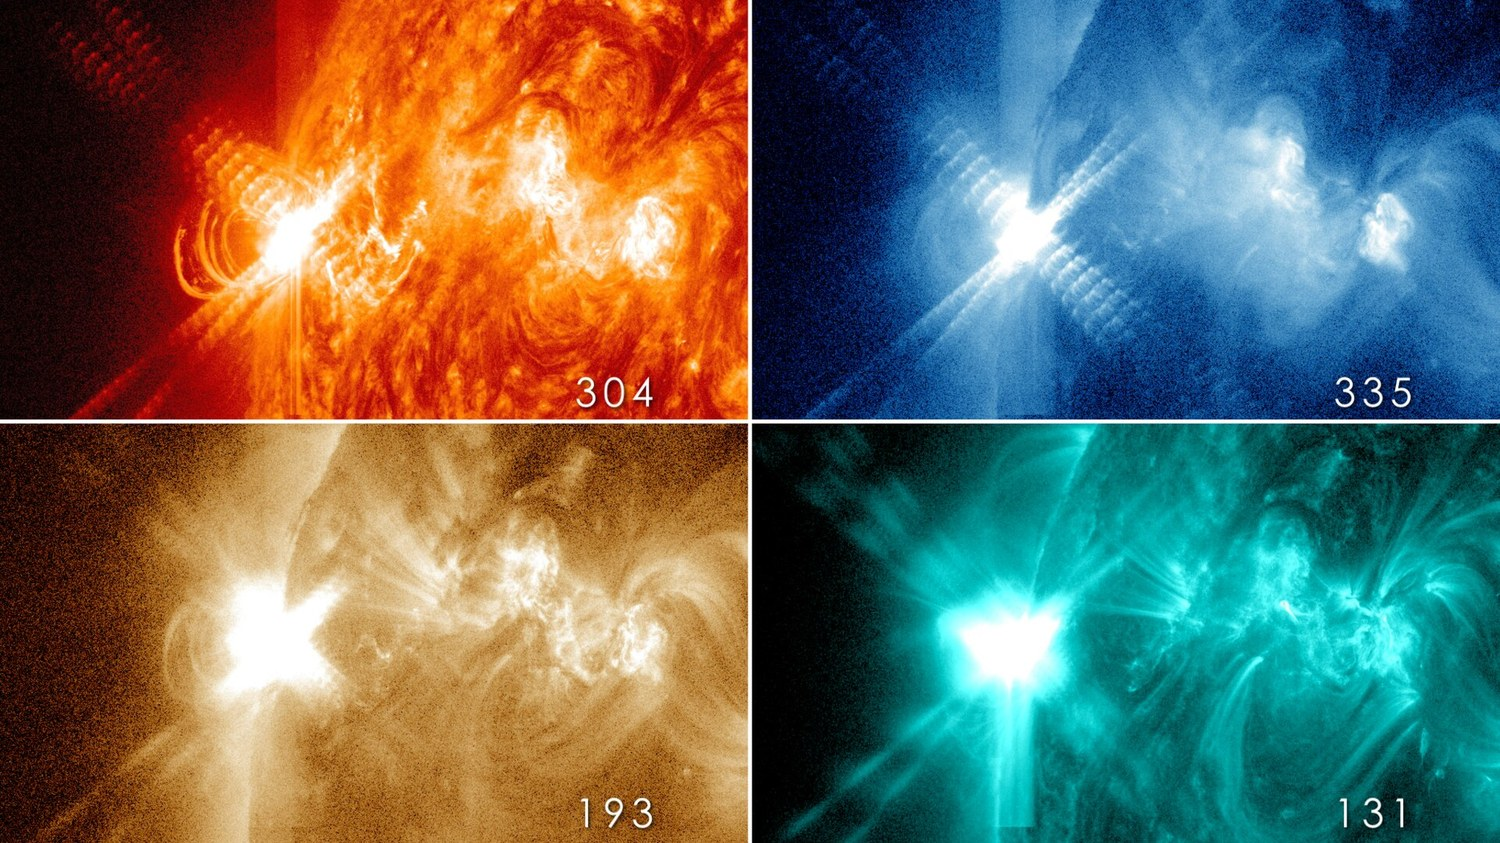
\includegraphics[width=0.72\textwidth]{../figures/solar_flare_sdo.jpg}
\caption{太阳耀斑：日冕里的磁重联现场。四个波段同时成像的耀斑是磁重联最直接的天然实验室：磁力线重排把磁能在几十分钟里放成热能与高能粒子，本节算的弓激波与磁鞘耗散、重联速率，在太阳大气里每天都在上演。}
\label{fig:photo-appab}
\figsource{NASA/SDO，Public domain（Wikimedia Commons）}
\end{figure}

\section{磁层对流与发电机：重联驱动的循环}
\label{sec:app-ab-convection}

磁层里的等离子体不静止：太阳风的电场把磁力线拖着走，形成\textbf{对流循环}。
在理想磁流体力学里，流动与磁场锁在一起，感生电场就是

\begin{equation}
\mathbf{E}=-\mathbf{v}\times\mathbf{B}.
\label{eq:app-ab-emf}
\end{equation}

代入 $v=400\ \mathrm{km\,s^{-1}}$、$B=5\ \mathrm{nT}$（垂直分量取 $1\ \mathrm{nT}$ 量级），
跨越 $10\ R_E$ 的电位差是几十千伏量级——这正是极区电离层被加速的能量来源。
把循环闭合起来靠的是\textbf{重联}：向阳面磁力线被压到一起并断开，磁尾里再合上，
于是磁力线从「日侧」被搬到了「夜侧」，等离子体跟着一起走。

发电机的严谨说法是欧姆定律的极限。等离子体的电导是阿尔芬电导

\begin{equation}
\Sigma_A=\frac{1}{\mu_0 v_A}=16.316\ \mathrm{S},
\label{eq:app-ab-sigma}
\end{equation}

只要它比碰撞电导大得多，「磁冻结」就成立，式 \eqref{eq:app-ab-emf} 才可以用。
电离层的佩德森电导只有 $1$--$10\ \mathrm{S}$ 量级，
两者串联决定了电流在哪里闭合——这叫\textbf{电离层发电机}。

\begin{table}[htbp]
\centering
\small
\begin{tabular}{p{3.2cm}p{3.2cm}p{3.4cm}p{4.0cm}}
\toprule
环节 & 关键量 & 数值 & 物理 \\
\midrule
对流电场 & $E=vB$ & 几十 $\mathrm{kV}$ / $10\ R_E$ & 太阳风拖磁力线 \\
阿尔芬电导 & $1/(\mu_0v_A)$ & $16.316\ \mathrm{S}$ & 磁冻结成立 \\
电离层电导 & 佩德森电导 & $1$--$10\ \mathrm{S}$ 量级 & 电流闭合 \\
循环闭合 & 重联 & 见 AB.5 & 日侧断开、夜侧合上 \\
\bottomrule
\end{tabular}
\caption{磁层对流链上的四个环节。本表把实验室里的「发电机」翻译成天体里的电流闭合问题。}
\label{tab:app-ab-convection}
\end{table}

\begin{tip}{发电机不是机器，是欧姆定律的一个极限}{tip-app-ab-dynamo}
教科书里的发电机是转子加线圈。等离子体里的「发电机」没有活动部件，它只是说：
\textbf{在电导足够大的极限下，流动必然感生电场，而电场又必须靠电流闭合}。
太阳风—磁层—电离层这条链之所以叫发电机，是因为它完成了同样的功能（把机械能变成电能耗散），
但机理完全不同：这里是磁冻结与电流守恒，不是电磁感应定律的应用题。
\end{tip}

{\footnotesize
\textbf{出处：}对流循环与电离层发电机的讲解参照 Kivelson \& Russell \emph{Introduction to Space Physics}
（1995，第 5--8 章）与 Baumjohann \& Treumann（1996，第 7、9 章）。
「欧姆定律极限」的表述方式参照 Priest \& Forbes \emph{Magnetic Reconnection}（2000，第 1--2 章）。
}

\section{磁重联：Sweet--Parker 与 Petschek 差在哪}
\label{sec:app-ab-reconnection}

对流循环要闭合，磁力线必须\textbf{断开再合上}。这一步叫磁重联，
它的全部困难可以用一个数说完——伦德奎斯特数

\begin{equation}
S=\frac{\mu_0 L v_A}{\eta},
\label{eq:app-ab-lundquist}
\end{equation}

其中 $\eta$ 是斯皮策电阻率。取重联区 $L=10^{6}\ \mathrm{m}$、$T=10\ \mathrm{eV}$、
库仑对数 $\ln\Lambda=20$，则

\begin{equation}
\eta=3.28877\times10^{-5}\ \Omega\,\mathrm{m},\qquad
S=1.86362\times10^{10}.
\label{eq:app-ab-eta}
\end{equation}

$S$ 巨大意味着磁场「粘」得厉害：扩散时间比阿尔芬时间大 $1.86362\times10^{10}$ 倍。
Sweet--Parker 模型让入流从整个长度 $L$ 上收进来，得到

\begin{equation}
\frac{v_{in}}{v_A}\sim S^{-1/2}=7.32523\times10^{-6},
\label{eq:app-ab-sp}
\end{equation}

对应的重联时间是

\begin{equation}
\tau_{SP}=\frac{L}{S^{-1/2}v_A}=2.79897\times10^{7}\ \mathrm{s}\;(323.95\ \text{天}),
\label{eq:app-ab-sptime}
\end{equation}

而太阳观测到的耀斑在分钟到小时量级——差五个数量级。
Petschek 把入流区压成一个小角，让出流几乎不受限：

\begin{equation}
\frac{v_{in}}{v_A}\sim\frac{\pi}{8\ln S}=0.0166058,
\label{eq:app-ab-petschek}
\end{equation}

比 Sweet--Parker 快 $2266.9$ 倍，重联时间落到 $12347\ \mathrm{s}$（约 $3.4$ 小时）量级。

\begin{table}[htbp]
\centering
\small
\begin{tabular}{p{3.2cm}p{3.0cm}p{3.2cm}p{3.8cm}}
\toprule
量 & 数值 & 单位 & 说明 \\
\midrule
斯皮策电阻率 $\eta$ & $3.28877\times10^{-5}$ & $\Omega\,\mathrm{m}$ & $T=10\ \mathrm{eV}$，$\ln\Lambda=20$ \\
伦德奎斯特数 $S$ & $1.86362\times10^{10}$ & --- & $L=10^6\ \mathrm{m}$ \\
Sweet--Parker 率 & $7.32523\times10^{-6}$ & --- & $S^{-1/2}$ \\
Petschek 率 & $0.0166058$ & --- & $\pi/(8\ln S)$ \\
两者之比 & $2266.9$ & --- & 快重联的全部理由 \\
Sweet--Parker 时间 & $2.79897\times10^{7}$ & $\mathrm{s}$ & $323.95$ 天 \\
Petschek 时间 & $12347$ & $\mathrm{s}$ & 约 $3.4$ 小时 \\
\bottomrule
\end{tabular}
\caption{两种重联模型在同一工作点下的对比。差别不在几何细节，而在入流面积。}
\label{tab:app-ab-reconnection}
\end{table}

\begin{tip}{电阻不够，重联靠的是「反常电阻」}{tip-app-ab-anomalous}
把式 \eqref{eq:app-ab-sp} 与观测对比会得到结论：真实的磁重联\textbf{不可能}只靠斯皮策电阻。
$S^{-1/2}=7.32523\times10^{-6}$ 意味着重联要 $323.95$ 天，而耀斑只给几分钟。
出路是局部的\textbf{反常电阻}：电流片薄到离子回旋半径量级时，
波与粒子相互作用接管了耗散，等效电阻率比斯皮策值大几个数量级，
$S$ 掉下来，重联率上去。所以「重联率是多少」这个问题，
在天体里往往等价于「耗散区有多薄」。
\end{tip}

{\footnotesize
\textbf{出处：}本节公式与两模型对比参照 Priest \& Forbes \emph{Magnetic Reconnection}
（2000，第 1--4 章）与 Kivelson \& Russell（1995，第 8 章）。
原始图像分别见 Sweet（1958）与 Petschek（1964）的会议文集。
无碰撞重联的定性说明参照 Baumjohann \& Treumann（1996，第 9 章）。
\textbf{不复制}原书推导与观测图，数值全部由 \texttt{tools/\allowbreak{}calc/\allowbreak{}appAB\_calc.py} 现算。
}

\section{辐射带与空间天气：磁矩守恒的必然结果}
\label{sec:app-ab-radbelt}

带电粒子在磁场里回旋，回旋半径

\begin{equation}
r_g=\frac{p_\perp}{|q|B}.
\label{eq:app-ab-larmor}
\end{equation}

取磁尾瓣典型的 $B=1.0\times10^{-7}\ \mathrm{T}$、粒子为 $1\ \mathrm{MeV}$ 电子，
动量 $p=7.59941\times10^{-22}\ \mathrm{kg\,m\,s^{-1}}$，于是

\begin{equation}
r_g=\frac{p}{eB}=47431.8\ \mathrm{m}\;(47.432\ \mathrm{km}).
\label{eq:app-ab-rg}
\end{equation}

$47\ \mathrm{km}$ 相比 $10\ R_E$ 很小——这就是「单粒子图像够用」的条件。
若换成太阳风中的电子（$B=5\ \mathrm{nT}$），回旋周期只有

\begin{equation}
T_{ce}=\frac{2\pi m_e}{eB}=0.00714477\ \mathrm{s},
\label{eq:app-ab-tce}
\end{equation}

即 $140\ \mathrm{Hz}$ 量级，远快于流体时间尺度。

回旋只是三层运动的第一层。粒子还沿磁力线来回弹跳、绕地球漂移，三者时间尺度分离时，
\textbf{磁矩 $\mu=p_\perp^2/(2mB)$ 近似守恒}。守恒的直接后果是\textbf{损失锥}：

\begin{equation}
\sin^2\alpha_c=\frac{B_{eq}}{B_{min}},
\label{eq:app-ab-losscone}
\end{equation}

投掷角小于 $\alpha_c$ 的粒子会撞进大气层损失掉，而 $B_{min}$ 越低锥越大——
磁暴期间磁场被压扁，损失锥张开，辐射带粒子被清空，这就是空间天气的物理内容。

\begin{table}[htbp]
\centering
\small
\begin{tabular}{p{2.6cm}p{3.2cm}p{3.2cm}p{4.2cm}}
\toprule
区域 & 主要粒子 & 关键尺度 & 主导物理 \\
\midrule
内辐射带 & 质子与高能电子 & $r_g$ 小、寿命长 & 磁矩守恒、CRAND 源 \\
外辐射带 & $1\ \mathrm{MeV}$ 电子 & $r_g=47.432\ \mathrm{km}$ & 波粒相互作用、加速 \\
槽区 & 电子通量低 & 损失与输运平衡 & 磁层对流与波散射 \\
磁尾瓣 & 等离子体片 & $B=1.0\times10^{-7}\ \mathrm{T}$ & 重联储能与释放 \\
\bottomrule
\end{tabular}
\caption{辐射带与磁尾的分区。本表只给尺度关系，不给通量数值。}
\label{tab:app-ab-radbelt}
\end{table}

\begin{tip}{辐射带不是「带」，是磁矩守恒的必然结果}{tip-app-ab-radbelt}
「带」这个字容易让人以为粒子被装在一个环形容器里。
真实图像相反：粒子只是\textbf{被磁矩守恒禁闭}——回旋半径远小于系统，
沿磁力线的运动又受磁镜力反射，于是它自然地留在一片L壳上。
所以辐射带的位置由磁场几何决定，强度由源与损失决定，
而「带」的形状在磁暴中会整体变形。把辐射带当成容器，就会看不懂它为什么会被一场磁暴清空。
\end{tip}

{\footnotesize
\textbf{出处：}三层运动与损失锥的讲解参照 Kivelson \& Russell \emph{Introduction to Space Physics}
（1995，第 3、10 章）与 Parks \emph{Physics of Space Plasmas}（2004，第 4、6 章）。
表 \ref{tab:app-ab-radbelt} 的四行内容由本文自拟，只给尺度关系不给通量，
数值由 \texttt{tools/\allowbreak{}calc/\allowbreak{}appAB\_calc.py} 复算，\textbf{不复制}原书的辐射带通量图。
}

\section{估算练习}
\label{sec:app-ab-problems}

下面六题只用本附录的公式与工作点，把其中一个量换掉重算一遍。

\textbf{练习 1}（密度）：把太阳风密度从 $5\ \mathrm{cm^{-3}}$ 加倍到 $10\ \mathrm{cm^{-3}}$，
温度、磁场与速度不变。求电子与离子等离子体频率、阿尔芬速与阿尔芬马赫数。

\textbf{练习 2}（温度）：温度升到 $100\ \mathrm{eV}$，其余不变。求声速、声速马赫数与 $\beta$。

\textbf{练习 3}（磁场）：磁场升到 $50\ \mathrm{nT}$。求阿尔芬速、阿尔芬马赫数与 $\beta$，
并说明为什么 $M_A$ 会掉到 $1$ 以下。

\textbf{练习 4}（重联区）：把重联区长度从 $10^{6}\ \mathrm{m}$ 缩到 $10^{4}\ \mathrm{m}$。
求伦德奎斯特数、Sweet--Parker 重联率与重联时间。

\textbf{练习 5}（辐射带）：把 1 MeV 电子换成 1 MeV 质子，磁场仍取 $1.0\times10^{-7}\ \mathrm{T}$。
求动量与回旋半径，并与电子的 $47.432\ \mathrm{km}$ 比较。

\textbf{练习 6}（功率）：太阳风速度加倍到 $800\ \mathrm{km\,s^{-1}}$，求输入磁层的功率。

\textbf{解答 1}：$\omega_{pe}=178399\ \mathrm{rad\,s^{-1}}$、$\omega_{pi}=4163.29\ \mathrm{rad\,s^{-1}}$、
$v_A=34.4879\ \mathrm{km\,s^{-1}}$、$M_A=11.5983$。
两个频率都涨 $\sqrt{2}$ 倍，而 $v_A$ 降 $\sqrt{2}$ 倍——密度同时进了两个地方，方向相反。

\textbf{解答 2}：$c_s=138.411\ \mathrm{km\,s^{-1}}$、$M_s=2.88994$、$\beta=8.05342$。
声速与 $\beta$ 都正比于 $T$ 的 $1/2$ 与 $1$ 次幂，温度一涨，太阳风就从强超声速退到弱超声速。

\textbf{解答 3}：$v_A=487.732\ \mathrm{km\,s^{-1}}$、$M_A=0.820123$、$\beta=8.05342\times10^{-3}$。
$v_A$ 正比于 $B$，磁场涨十倍就把阿尔芬速抬到 $487.732\ \mathrm{km\,s^{-1}}$，超过流速，
于是 $M_A<1$：这种等离子体里阿尔芬波跑得比流动快，磁力线不再被「拖」着走。

\textbf{解答 4}：$S=1.86362\times10^{8}$、$S^{-1/2}=7.32523\times10^{-5}$、$\tau_{SP}=2798.97\ \mathrm{s}$（$46.6494$ 分钟）。
$S\propto L$，长度缩一百倍使重联率涨十倍、时间降到原来的十分之一——
但 $46.6494$ 分钟仍远长于耀斑的分钟量级，这就是必须引入反常电阻的原因。

\textbf{解答 5}：$p=2.3151\times10^{-20}\ \mathrm{kg\,m\,s^{-1}}$、$r_g=1444.97\ \mathrm{km}$。
同样 $1\ \mathrm{MeV}$，质子比电子重 $1836$ 倍，动量涨 $\sqrt{1836}\approx42.9$ 倍，
回旋半径从 $47.432\ \mathrm{km}$ 涨到 $1444.97\ \mathrm{km}$——这个尺度已经可以和磁层结构相比，
所以高能离子必须用单粒子轨道而不是流体描述。

\textbf{解答 6}：$P=2.73006\times10^{11}\ \mathrm{W}=273.006\ \mathrm{GW}$，是原值的 $8$ 倍。
因为功率 $\propto v^3$，速度加倍就涨八倍；这也是磁暴期间能量输入暴涨的原因。

\section{来源、分级与版权说明}
\label{sec:app-ab-source}

\begingroup\small
这一篇与 M--AA 那批「装置篇」不重叠：那些附录回答「装置怎么运行」，
这一篇回答「同一套方程在没有边界墙的地方长什么样」。
两者共享的物理是磁冻结、磁压与热压之比、以及重联；不共享的是边界条件。

\subsection*{借鉴来源（只写书名与年份，不写 DOI）}

\begin{table}[htbp]
\centering
\small
\begin{tabular}{p{4.4cm}p{1.8cm}p{6.6cm}}
\toprule
来源 & 年份 & 本附录用到的部分 \\
\midrule
Kivelson \& Russell《Introduction to Space Physics》 & 1995 & 尺度分区、磁层顶平衡、辐射带 \\
Baumjohann \& Treumann《Basic Space Plasma Physics》 & 1996 & 声速与阿尔芬速、无碰撞激波、重联入门 \\
Priest \& Forbes《Magnetic Reconnection》 & 2000 & Sweet--Parker 与 Petschek 两模型 \\
Parks《Physics of Space Plasmas》 & 2004 & 激波耗散、三层运动与损失锥 \\
Sweet (1958) / Petschek (1964) 会议文集 & 1958/1964 & 两种重联的原始图像 \\
\bottomrule
\end{tabular}
\caption{本附录借鉴的经典来源与各自被用到的部分。}
\label{tab:app-ab-source}
\end{table}

\subsection*{数值分级}

本附录的数字分三级，正文里逐节标明：

\begin{itemize}
\item \textbf{现算级}：由 \texttt{tools/\allowbreak{}calc/\allowbreak{}appAB\_calc.py} 现算并打印，与脚本输出逐位一致。
包括两个频率、声速、阿尔芬速、两个马赫数、$\beta$、动压与磁压、磁层顶距离、
输入功率、电阻率、伦德奎斯特数、两种重联率与时间、回旋半径与回旋周期、阿尔芬电导。
\item \textbf{声明级}：作为输入直接取定的四个数
（$n=5\ \mathrm{cm^{-3}}$、$T=10\ \mathrm{eV}$、$B=5\ \mathrm{nT}$、$v=400\ \mathrm{km\,s^{-1}}$）、
重联区的 $L=10^{6}\ \mathrm{m}$ 与 $\ln\Lambda=20$、磁尾瓣的 $B=1.0\times10^{-7}\ \mathrm{T}$。
这些不是结论，是工作点，换一组值结论会变。
\item \textbf{文献级}：只在定性句子里出现，不给具体数——观测到的磁层顶位置约 $10\ R_E$、
耀斑重联的分钟到小时量级、电离层佩德森电导 $1$--$10\ \mathrm{S}$。
它们的作用是提供量级对照，不参与复算。
\end{itemize}

\subsection*{版权口径}

本附录\textbf{不复制}任何原书的文字、公式编号、插图与数据表：
所有中文表述、表格版式与数值均由本文自拟并独立复算，
只在「借鉴来源」中标注物理结论与讲解顺序的出处。
本附录\textbf{不复制}任何观测通量数值——辐射带一节只给尺度关系，
原始观测文献没有逐一核对，这里只给量级。
\endgroup
